\part{Counting}
\section{Handout 01: Basics of Counting}

\subsection{Overview}

This handout introduces the basic counting language used throughout MH1301. The central lesson is not merely that one should know several formulas, but that one should first identify the \emph{right mathematical model} for the objects in the question. A counting problem becomes manageable only after it is written as a problem about sets, sequences, functions, binary strings, disjoint cases, or overlapping cases.

The core topics of this handout are:
\begin{itemize}[leftmargin=*]
    \item reminders on sets and cardinality;
    \item the distinction between sequences and sets;
    \item the product rule and permutations;
    \item counting functions between finite sets;
    \item injective, surjective, and bijective functions;
    \item counting by bijection;
    \item binary strings and subsets;
    \item the sum rule;
    \item inclusion--exclusion for two sets, three sets, and the general case.
\end{itemize}

\begin{examtip}[title={The guiding question of Handout 01}]
Before counting, ask: \emph{What is a single object here?} If you identify the object incorrectly, the rest of the calculation is usually wrong even if the arithmetic is flawless.
\end{examtip}

%==================================================
\subsection{Sets, Cardinality, and Counting}
%==================================================

\begin{definition}{Set and cardinality}{set-cardinality}
A \emph{set} is an unordered collection of objects, called its elements. If $S$ is finite, its \emph{cardinality} $|S|$ is the number of distinct elements in $S$.
\end{definition}

The set viewpoint matters because counting is fundamentally the task of determining the size of an explicitly defined set. Two reminders from elementary set theory are especially important in this chapter:
\begin{itemize}[leftmargin=*]
    \item the order in which elements are listed in a set is irrelevant;
    \item repeated listing does not create new elements.
\end{itemize}

Thus
\[
\{a,b,c\}=\{b,c,a\}=\{a,b,c,a\}
\qquad\text{and hence}\qquad
|\{a,b,c,a\}|=3.
\]

\begin{definition}{Subset}{subset}
If $A$ and $B$ are sets, then $A\subseteq B$ means that every element of $A$ is also an element of $B$.
\end{definition}

\begin{examplebox}[title={Why the notion of a set matters in counting}]
If a problem asks for the number of subsets of $\{1,2,3\}$, the objects being counted are
\[
\varnothing,\ \{1\},\ \{2\},\ \{3\},\ \{1,2\},\ \{1,3\},\ \{2,3\},\ \{1,2,3\}.
\]
The expressions $\{1,2\}$ and $\{2,1\}$ represent the same subset, so they should not be counted separately.
\end{examplebox}

\begin{commonmistake}[title={Counting symbols instead of distinct elements}]
The notation used to display a set is not the object itself. Repeated entries and reordered entries do not change the set. This is one of the earliest places where overcounting can happen.
\end{commonmistake}

%==================================================
\subsection{Sequences versus Sets}
%==================================================

\begin{definition}{Sequence}{sequence}
A \emph{sequence} is an ordered collection of elements, not necessarily distinct.
\end{definition}

This contrasts sharply with the notion of a set. In a sequence, position matters; in a set, it does not.

\begin{examplebox}[title={Basic contrast}]
The sequences
\[
(a,b,c),\qquad (b,a,c),\qquad (a,b,a)
\]
are generally different. By contrast,
\[
\{a,b,c\}=\{b,a,c\}
\]
as sets.
\end{examplebox}

\begin{examtip}[title={Recognition pattern}]
Words such as \emph{string}, \emph{code}, \emph{password}, \emph{arrangement}, \emph{line up}, and \emph{permutation} usually indicate that the relevant object is a sequence rather than a set.
\end{examtip}

%==================================================
\subsection{Product Rule}
%==================================================

\begin{theorem}{Product Rule}{product-rule}
Suppose a set $S$ consists of sequences of length $k$, where there are $n_1$ possible first entries, $n_2$ possible second entries for each first entry, and so on up to $n_k$ possible $k$-th entries for each compatible previous choice. Then
\[
|S|=n_1n_2\cdots n_k.
\]
\end{theorem}

The product rule is the rule for \emph{sequential construction}. It applies when an object can be built in stages and each stage has a known number of possibilities.

\begin{examplebox}[title={Die and coin}]
When a six-sided die and a two-sided coin are tossed together, an outcome is an ordered pair
\[
(\text{die outcome},\text{coin outcome}).
\]
There are $6$ choices for the first component and $2$ for the second, so the total number of outcomes is
\[
6\cdot 2=12.
\]
\end{examplebox}

\begin{examplebox}[title={License plates}]
If each plate consists of a sequence of $3$ letters followed by $3$ digits, then the number of possible plates is
\[
26^3\cdot 10^3=17{,}576{,}000.
\]
This is a direct product-rule problem because each position is filled in sequence.
\end{examplebox}

\begin{examplebox}[title={Tutorial 1, Question 1(a)}]
How many different three-letter initials are possible if there are $26$ letters?

\textbf{Solution.}
Each of the three positions may be filled by any of $26$ letters, so the total number is
\[
26^3=17{,}576.
\]
\end{examplebox}

\begin{extension}[title={Decision-tree viewpoint for the product rule}]
One can visualise the product rule using a decision tree: each level corresponds to one stage of the choice process, and each root-to-leaf path corresponds to one completed object. If every path has $n_1,n_2,\dots,n_k$ choices at the respective levels, then the total number of leaves is $n_1n_2\cdots n_k$.
\end{extension}

\begin{commonmistake}[title={Multiplying visible numbers without identifying stages}]
The product rule applies because an object is built step by step, not because several numbers happen to appear in the question. If the stages are not well defined, multiplication may be unjustified.
\end{commonmistake}

%==================================================
\subsection{Permutations}
%==================================================

\begin{definition}{Permutation}{permutation}
A \emph{permutation} of a finite set $S$ is a sequence containing every element of $S$ exactly once.
\end{definition}

\begin{theorem}{Number of permutations}{permutation-count}
If $|S|=n$, then the number of permutations of $S$ is
\[
n!.
\]
\end{theorem}

\begin{proof}
For the first position, there are $n$ choices. After choosing one element, there are $n-1$ choices for the second position, then $n-2$ for the third, and so on, until one choice remains for the last position. By the product rule,
\[
n(n-1)(n-2)\cdots 2\cdot 1=n!.
\]
\end{proof}

\begin{examplebox}[title={Permutations of $\{1,2,3\}$}]
The permutations are
\[
(1,2,3),\ (1,3,2),\ (2,1,3),\ (2,3,1),\ (3,1,2),\ (3,2,1),
\]
so there are $3!=6$ of them.
\end{examplebox}

\begin{examtip}[title={Recognition pattern for permutations}]
If a problem asks for orderings of distinct objects without repetition, factorial growth is usually present. Still, one should justify which objects occupy which positions rather than writing $n!$ immediately.
\end{examtip}

%==================================================
\subsection{Functions and Counting Functions}
%==================================================

\begin{definition}{Function}{function}
Let $X$ and $Y$ be sets. A function $f:X\to Y$ assigns to each element $x\in X$ exactly one element $f(x)\in Y$.
\end{definition}

\begin{examplebox}[title={What is and is not a function}]
The rule $f(x)=x^2$ is a function because each input has exactly one output. By contrast, the rule $f(x)=\pm\sqrt{x}$ is not a function from the nonnegative reals to the reals, because one input generally has two possible outputs.
\end{examplebox}

\begin{theorem}{Counting all functions}{count-functions}
If $|X|=m$ and $|Y|=n$, then the number of functions from $X$ to $Y$ is
\[
n^m.
\]
\end{theorem}

\begin{proof}
Each element of the domain $X$ independently chooses one image in $Y$. Since there are $m$ domain elements and $n$ choices for each, the product rule gives
\[
\underbrace{n\cdot n\cdots n}_{m\text{ times}}=n^m.
\]
\end{proof}

\begin{examplebox}[title={A function-counting model}]
If $|X|=4$ and $|Y|=3$, then each of the $4$ elements of $X$ chooses one of $3$ images in $Y$, so the number of functions $X\to Y$ is
\[
3^4=81.
\]
\end{examplebox}

\begin{commonmistake}[title={Why the answer is $n^m$, not $mn$}]
The quantity $mn$ would count ordered pairs $(x,y)$ with $x\in X$ and $y\in Y$, not functions from $X$ to $Y$. A function requires an image choice for \emph{every} element of the domain.
\end{commonmistake}

%==================================================
\subsection{Injective, Surjective, and Bijective Functions}
%==================================================

\begin{definition}{Injective, surjective, bijective}{inj-surj-bij}
Let $f:X\to Y$.
\begin{itemize}[leftmargin=*]
    \item $f$ is \emph{injective} if distinct elements of $X$ have distinct images.
    \item $f$ is \emph{surjective} if every element of $Y$ is the image of at least one element of $X$.
    \item $f$ is \emph{bijective} if it is both injective and surjective.
\end{itemize}
\end{definition}

% Fallback description: three simple mapping diagrams illustrating surjective/non-injective, injective/non-surjective, and bijective maps.
\begin{center}
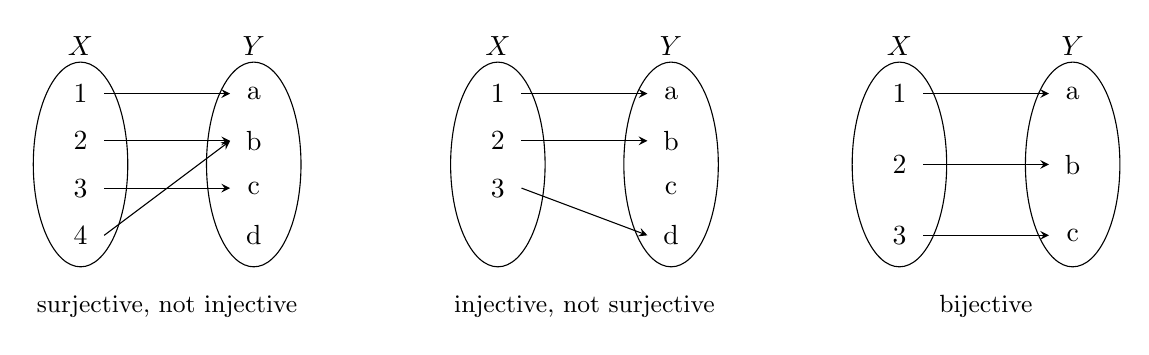
\begin{tikzpicture}[x=1cm,y=1cm,>=stealth]
    \draw (0,0) ellipse (0.6 and 1.3);
    \draw (2.2,0) ellipse (0.6 and 1.3);
    \node at (0,1.5) {$X$};
    \node at (2.2,1.5) {$Y$};
    \foreach \y/\lab in {0.9/1,0.3/2,-0.3/3,-0.9/4}
        \node at (0,\y) {\lab};
    \foreach \y/\lab in {0.9/a,0.3/b,-0.3/c,-0.9/d}
        \node at (2.2,\y) {\lab};
    \draw[->] (0.3,0.9) -- (1.9,0.9);
    \draw[->] (0.3,0.3) -- (1.9,0.3);
    \draw[->] (0.3,-0.3) -- (1.9,-0.3);
    \draw[->] (0.3,-0.9) -- (1.9,0.3);
    \node at (1.1,-1.8) {\small surjective, not injective};

    \begin{scope}[shift={(5.3,0)}]
        \draw (0,0) ellipse (0.6 and 1.3);
        \draw (2.2,0) ellipse (0.6 and 1.3);
        \node at (0,1.5) {$X$};
        \node at (2.2,1.5) {$Y$};
        \foreach \y/\lab in {0.9/1,0.3/2,-0.3/3}
            \node at (0,\y) {\lab};
        \foreach \y/\lab in {0.9/a,0.3/b,-0.3/c,-0.9/d}
            \node at (2.2,\y) {\lab};
        \draw[->] (0.3,0.9) -- (1.9,0.9);
        \draw[->] (0.3,0.3) -- (1.9,0.3);
        \draw[->] (0.3,-0.3) -- (1.9,-0.9);
        \node at (1.1,-1.8) {\small injective, not surjective};
    \end{scope}

    \begin{scope}[shift={(10.4,0)}]
        \draw (0,0) ellipse (0.6 and 1.3);
        \draw (2.2,0) ellipse (0.6 and 1.3);
        \node at (0,1.5) {$X$};
        \node at (2.2,1.5) {$Y$};
        \foreach \y/\lab in {0.9/1,0.0/2,-0.9/3}
            \node at (0,\y) {\lab};
        \foreach \y/\lab in {0.9/a,0.0/b,-0.9/c}
            \node at (2.2,\y) {\lab};
        \draw[->] (0.3,0.9) -- (1.9,0.9);
        \draw[->] (0.3,0.0) -- (1.9,0.0);
        \draw[->] (0.3,-0.9) -- (1.9,-0.9);
        \node at (1.1,-1.8) {\small bijective};
    \end{scope}
\end{tikzpicture}
\end{center}

\begin{theorem}{Cardinality constraints for finite sets}{map-cardinality}
Let $X$ and $Y$ be finite sets and let $f:X\to Y$.
\begin{itemize}[leftmargin=*]
    \item If $f$ is injective, then $|X|\le |Y|$.
    \item If $f$ is surjective, then $|X|\ge |Y|$.
    \item If $f$ is bijective, then $|X|=|Y|$.
\end{itemize}
\end{theorem}

These facts are often called mapping rules. They are especially useful because they allow set sizes to be compared without counting both sets directly.

\begin{extension}[title={Bijections are exact counting transfers}]
A bijection does more than show two sets have the same size abstractly. It gives a one-to-one translation between their elements. In counting problems this matters because it guarantees that no object is lost and no object is counted twice.
\end{extension}

%==================================================
\subsection{Counting via Bijection}
%==================================================

\begin{definition}{Counting by bijection}{counting-bijection}
To count a difficult finite set $A$, one may construct a bijection from $A$ to a simpler finite set $B$. Since bijections preserve cardinality,
\[
|A|=|B|.
\]
\end{definition}

This is one of the most powerful ideas in discrete mathematics. Often the original objects are awkward, but a good encoding turns them into strings, subsets, or functions that can be counted immediately.

\begin{examtip}[title={Bijection checklist}]
When using a bijection, verify three things explicitly:
\begin{enumerate}[leftmargin=*]
    \item the encoding is well defined;
    \item different original objects cannot map to the same code;
    \item every valid code comes from an original object.
\end{enumerate}
\end{examtip}

%==================================================
\subsection{Binary Strings and Subsets}
%==================================================

\begin{definition}{Binary string}{binary-string}
An \emph{$n$-bit binary string} is a sequence $(b_1,\dots,b_n)$ in which each $b_i\in\{0,1\}$.
\end{definition}

\begin{theorem}{Counting binary strings}{count-binary}
The number of binary strings of length $n$ is
\[
2^n.
\]
\end{theorem}

\begin{proof}
Each of the $n$ positions has two possible entries, $0$ or $1$. By the product rule, the total number of strings is $2^n$.
\end{proof}

\begin{examplebox}[title={Tutorial 1, Question 2(b)}]
How many bit strings of length $n$ start and end with $1$?

\textbf{Solution.}
If $n=1$, there is exactly one such string, namely $1$.
For $n\ge 2$, the first and last positions are fixed, and the remaining $n-2$ positions are arbitrary. Hence the number is
\[
2^{n-2}\qquad (n\ge 2).
\]
\end{examplebox}

\begin{theorem}{Number of subsets of a finite set}{power-set-count}
If $S=\{1,2,\dots,n\}$, then the number of subsets of $S$ is
\[
2^n.
\]
\end{theorem}

\begin{proof}
Associate to each subset $A\subseteq S$ the binary string $(b_1,\dots,b_n)$ defined by
\[
b_i=
\begin{cases}
1,& i\in A,\\
0,& i\notin A.
\end{cases}
\]
This is a bijection between subsets of $S$ and binary strings of length $n$. Since there are $2^n$ such strings, there are $2^n$ subsets of $S$.
\end{proof}

% Fallback description: subset-to-binary-string encoding showing membership positions.
\begin{center}
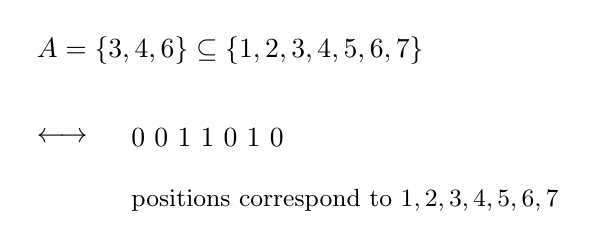
\begin{tikzpicture}[x=1cm,y=1cm]
    \node[anchor=west] at (0,1.1) {$A=\{3,4,6\}\subseteq \{1,2,3,4,5,6,7\}$};
    \node[anchor=west] at (0,0) {$\longleftrightarrow$};
    \node[anchor=west] at (1.2,0) {$0\ 0\ 1\ 1\ 0\ 1\ 0$};
    \node[anchor=west] at (1.2,-0.8) {\small positions correspond to $1,2,3,4,5,6,7$};
\end{tikzpicture}
\end{center}

\begin{examplebox}[title={The standard subset encoding}]
For $S=\{1,2,3,4,5,6,7\}$, the subset $\{3,4,6\}$ corresponds to the string
\[
(0,0,1,1,0,1,0),
\]
because positions $3$, $4$, and $6$ are marked by $1$.
\end{examplebox}

\begin{extension}[title={Characteristic-function viewpoint}]
The binary-string encoding of a subset $A\subseteq S$ can also be viewed as its characteristic function
\[
\chi_A:S\to\{0,1\},
\qquad
\chi_A(s)=
\begin{cases}
1,& s\in A,\\
0,& s\notin A.
\end{cases}
\]
So subset counting is also a function-counting problem: each element of $S$ independently chooses one of two possible outputs.
\end{extension}

%==================================================
\subsection{Sum Rule}
%==================================================

\begin{theorem}{Sum Rule}{sum-rule}
If $A_1,\dots,A_k$ are pairwise disjoint finite sets, then
\[
|A_1\cup\cdots\cup A_k|=|A_1|+\cdots+|A_k|.
\]
\end{theorem}

The sum rule applies when the total collection has been partitioned into disjoint cases. Each object belongs to exactly one case, so simple addition is valid.

\begin{examplebox}[title={Textbooks}]
If there are $26$ MH1301 textbooks in one library and $15$ in another, and the two collections are taken as disjoint holdings, then the total number is
\[
26+15=41.
\]
\end{examplebox}

\begin{examplebox}[title={Passwords of lengths 6, 7, or 8}]
Suppose a password consists of uppercase letters or digits and has length $6$, $7$, or $8$. There are $26+10=36$ choices for each character. Let $X_6$, $X_7$, and $X_8$ denote the sets of passwords of lengths $6$, $7$, and $8$. These sets are disjoint, so
\[
|X_6\cup X_7\cup X_8|=|X_6|+|X_7|+|X_8|=36^6+36^7+36^8.
\]
\end{examplebox}

\begin{extension}[title={Why naive sum rule fails with overlap}]
The equation $|A\cup B|=|A|+|B|$ is not a general union formula; it is a \emph{disjoint-union} formula. The moment one object can satisfy both case descriptions, addition alone overcounts that object.
\end{extension}

\begin{commonmistake}[title={Using ``or'' as a signal for addition}]
The word \emph{or} does not by itself justify the sum rule. One must still check whether the cases are disjoint. If they overlap, the correct tool is inclusion--exclusion or a finer disjoint partition.
\end{commonmistake}

%==================================================
\subsection{Inclusion--Exclusion for Two Sets}
%==================================================

\begin{theorem}{Two-set inclusion--exclusion}{ie-two}
For any finite sets $A$ and $B$,
\[
|A\cup B|=|A|+|B|-|A\cap B|.
\]
\end{theorem}

\begin{proof}
In the sum $|A|+|B|$, elements of $A\setminus B$ and $B\setminus A$ are counted once, while elements of $A\cap B$ are counted twice. Subtracting $|A\cap B|$ corrects the double counting.
\end{proof}

% Fallback description: two-set Venn diagram indicating that the overlap is the region counted twice before correction.
\begin{center}
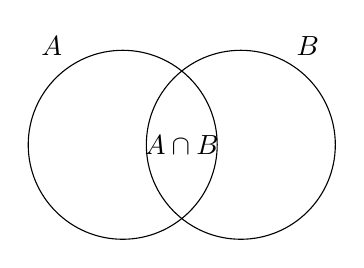
\begin{tikzpicture}[scale=1]
    \draw (0,0) circle (1.2);
    \draw (1.5,0) circle (1.2);
    \node at (-0.9,1.25) {$A$};
    \node at (2.35,1.25) {$B$};
    \node at (0.75,0) {$A\cap B$};
\end{tikzpicture}
\end{center}

\begin{examplebox}[title={Bit strings of length 8}]
How many $0$-$1$ strings of length $8$ either start with $1$ or end with $00$?

\textbf{Solution.}
Let
\[
A=\{\text{strings starting with }1\},
\qquad
B=\{\text{strings ending with }00\}.
\]
Then
\[
|A|=2^7=128,
\qquad
|B|=2^6=64.
\]
Also,
\[
|A\cap B|=2^5=32,
\]
because such a string has the form
\[
1\ \square\ \square\ \square\ \square\ \square\ 0\ 0.
\]
Hence
\[
|A\cup B|=128+64-32=160.
\]
\end{examplebox}

\begin{examplebox}[title={Students taking Mathematics or Physics}]
Suppose there are $1807$ students in total, with $453$ taking Mathematics, $567$ taking Physics, and $299$ taking both. Then the number taking at least one of the two subjects is
\[
453+567-299=721.
\]
Therefore the number taking neither is
\[
1807-721=1086.
\]
\end{examplebox}

\begin{extension}[title={Indicator-style intuition for the two-set formula}]
For each object $x$, the indicator of membership in $A\cup B$ satisfies
\[
1_{A\cup B}(x)=1_A(x)+1_B(x)-1_{A\cap B}(x).
\]
Summing this identity over all objects in the universe gives the cardinality formula. This viewpoint explains inclusion--exclusion as a pointwise correction mechanism rather than a formula to memorise blindly.
\end{extension}

%==================================================
\subsection{Inclusion--Exclusion for Three Sets}
%==================================================

\begin{theorem}{Three-set inclusion--exclusion}{ie-three}
For finite sets $A$, $B$, and $C$,
\[
|A\cup B\cup C|
=
|A|+|B|+|C|
-|A\cap B|-|A\cap C|-|B\cap C|
+|A\cap B\cap C|.
\]
\end{theorem}

\begin{proof}
The first three terms count every element once for each set containing it. Thus an element in exactly two sets is counted twice and must be corrected by subtracting the relevant pairwise intersection. But an element in all three sets is then subtracted three times after being added three times, so it must be added back once.
\end{proof}

% Fallback description: three-set Venn diagram highlighting the central triple-overlap region that is added back at the last step.
\begin{center}
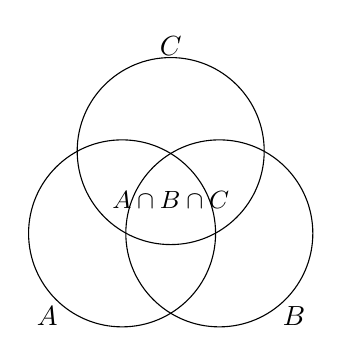
\begin{tikzpicture}[scale=0.95]
    \draw (0,0) circle (1.25);
    \draw (1.3,0) circle (1.25);
    \draw (0.65,1.1) circle (1.25);
    \node at (-1.0,-1.1) {$A$};
    \node at (2.3,-1.1) {$B$};
    \node at (0.65,2.5) {$C$};
    \node at (0.65,0.45) {\small $A\cap B\cap C$};
\end{tikzpicture}
\end{center}

\begin{examplebox}[title={Spanish, French, and Russian courses}]
Suppose
\[
|S|=1232,\quad |F|=879,\quad |R|=114,
\]
\[
|S\cap F|=103,\quad |S\cap R|=23,\quad |F\cap R|=14,
\]
and
\[
|S\cup F\cup R|=2092.
\]
Then
\[
2092=1232+879+114-103-23-14+|S\cap F\cap R|,
\]
so
\[
|S\cap F\cap R|=7.
\]
\end{examplebox}

\begin{extension}[title={Why the signs alternate}]
Inclusion--exclusion alternates signs because each stage corrects the overcorrection from the previous stage. First the single-set counts overcount overlaps, then pairwise subtraction overcorrects the deepest overlaps, then triple intersections restore the correct count, and so on.
\end{extension}

%==================================================
\subsection{General Inclusion--Exclusion Principle}
%==================================================

\begin{theorem}{General inclusion--exclusion principle}{ie-general}
For finite sets $A_1,\dots,A_n$,
\[
\left|\bigcup_{i=1}^n A_i\right|
=
\sum_{i=1}^n |A_i|
-
\sum_{1\le i<j\le n}|A_i\cap A_j|
+
\sum_{1\le i<j<k\le n}|A_i\cap A_j\cap A_k|
-\cdots+
(-1)^{n-1}|A_1\cap\cdots\cap A_n|.
\]
\end{theorem}

A useful verbal memory pattern is:
\begin{center}
add the single-set sizes, subtract the two-way intersections, add the three-way intersections, subtract the four-way intersections, and continue alternating.
\end{center}

\begin{proof}[Sketch of proof]
The standard proof is by induction on $n$.
For $n=1$ and $n=2$, the statement is immediate.
Assume the formula holds for $n$ sets. Then
\[
\bigcup_{i=1}^{n+1}A_i
=
\left(\bigcup_{i=1}^n A_i\right)\cup A_{n+1}.
\]
Applying the two-set inclusion--exclusion formula gives
\[
\left|\bigcup_{i=1}^{n+1}A_i\right|
=
\left|\bigcup_{i=1}^{n}A_i\right|+|A_{n+1}|-
\left|\left(\bigcup_{i=1}^{n}A_i\right)\cap A_{n+1}\right|.
\]
Now use the identity
\[
\left(\bigcup_{i=1}^{n}A_i\right)\cap A_{n+1}
=
\bigcup_{i=1}^{n}(A_i\cap A_{n+1}),
\]
and apply the inductive hypothesis to the two unions. The alternating-sign pattern is preserved, giving the formula for $n+1$ sets.
\end{proof}

\begin{extension}[title={Canonical correction viewpoint}]
General inclusion--exclusion can be understood as a correction algorithm: count everything that qualifies at least once, then remove overcounts, then repair the over-repair, and continue until every object that belongs to the union has net weight exactly $1$.
\end{extension}

%==================================================
\subsection{Special Techniques and Elegant Problem-Solving Ideas}
%==================================================

\subsubsection*{Counting by bijection}
A difficult family of objects is often easier to count after a clean encoding into binary strings, subsets, or functions. The value of a bijection is that it turns a conceptual observation into an exact counting statement.

\subsubsection*{Binary encoding of subsets}
Whenever each labelled element may either be chosen or not chosen, a binary model is natural. This is the fastest route to the formula $2^n$ for subsets of an $n$-element set.

\subsubsection*{Complement counting}
If the desired class is hard to count directly but the excluded class is simple, count the universe and subtract the complement. This frequently appears in string-counting questions involving conditions such as ``at least one'' or ``not all''.

\subsubsection*{Partition before using the sum rule}
If the cases initially overlap, refine them into genuinely disjoint subcases before adding. This is often a cleaner alternative to applying inclusion--exclusion immediately.

\subsubsection*{Detect overlap before counting}
Before adding case counts, always ask whether one object can satisfy two of the case descriptions simultaneously. If yes, direct addition is unsafe.

\subsubsection*{Convert objects into strings or functions}
Many combinatorial objects are best thought of as a finite sequence of labelled decisions. Once the positions and choices are identified, the product rule often becomes immediate.

\begin{examtip}[title={A practical hierarchy of methods for Handout 01}]
For a new counting problem, a good order of attack is:
\begin{enumerate}[leftmargin=*]
    \item try to model the object directly as a sequence of choices;
    \item if cases split naturally, test whether they are disjoint;
    \item if overlap appears, use inclusion--exclusion or refine the partition;
    \item if the objects remain awkward, search for a bijection to a cleaner family.
\end{enumerate}
\end{examtip}

%==================================================
\subsection{Final Consolidation}
%==================================================

\begin{center}
\small
\begin{tabular}{@{}p{0.25\textwidth}p{0.28\textwidth}p{0.37\textwidth}@{}}
\toprule
\textbf{Situation} & \textbf{Primary tool} & \textbf{Typical signal words} \\
\midrule
Sequential choices & Product rule & choose, then, fill positions, assign \\
Ordered arrangement without repetition & Permutations & arrange, order, line up, rank \\
Functions from one finite set to another & Function counting & map each element, assign outputs \\
Equivalent easier model & Bijection & encode, represent, correspond \\
Yes/no choice per label & Binary strings & subset, selected/not selected \\
Disjoint cases & Sum rule & either this case or that case, by length, by type \\
Overlapping cases & Inclusion--exclusion & overlap, at least one, counted twice \\
\bottomrule
\end{tabular}
\end{center}

\begin{commonmistake}[title={Final checklist for Handout 01}]
Before accepting a counting solution, verify:
\begin{enumerate}[leftmargin=*]
    \item Have I identified the objects correctly as sets, sequences, or functions?
    \item Have I justified why the chosen rule applies?
    \item If I used the sum rule, are the cases disjoint?
    \item If I used inclusion--exclusion, did I count the overlap correctly?
    \item If I used a bijection, did I explain why it is one-to-one and onto?
\end{enumerate}
\end{commonmistake}

\begin{examtip}[title={What should remain after this handout}]
After Handout 01, the main skills to retain are: modelling a counting problem as a set problem, recognising when order matters, using the product rule and sum rule correctly, correcting overlap by inclusion--exclusion, and translating objects into easier forms through bijections and binary encodings.
\end{examtip}